\section{Аналитическая часть}
\label{sec:anal}

В аналитической части собраны стратегия и состав автоматических тестов, метрики
покрытия кода и числа сравнительных прогонов с двумя альтернативными реализациями языка.
По ним проверяется две вещи: что реализация ведёт себя так, как задумано в конструкторской
части (раздел~\ref{sec:design}), и что измеренная производительность совпадает с
теоретическими ожиданиями из раздела~\ref{sec:research}.

\subsection{Стратегия тестирования}
\label{subsec:test-strategy}

Тесты разбиты на три уровня по характеру проверяемого поведения.

\textbf{Юнит-тесты} проверяют отдельные компоненты в изоляции: раскрученную
двустороннюю очередь (\prog{ShallowDeque}, \prog{DeepDeque}, \prog{ExprOps.concat}),
лексер, парсер, семантический анализ, сопоставитель шаблонов,
конструктор результата и встроенные функции.

\textbf{Интеграционные тесты} прогоняют полную цепочку «разбор
$\to$ семантика $\to$ нормализация» на предготовленных фикстурах:
фиксируется конкретный вывод интерпретатора и коды возврата CLI.

\textbf{Тесты совместимости} (\prog{AutotestsRunnerTest}) запускают
интерпретатор как внешний процесс на наборах тестовых программ, унаследованных
от существующих реализаций Рефала, и проверяют результаты построчно.

В качестве фреймворка используется JUnit~5~\cite{junit5_guide};
все сравнения~--- через AssertJ~\cite{assertj_docs};
покрытие кода~--- JaCoCo~\cite{jacoco_docs}.

\subsection{Состав тестов}
\label{subsec:test-counts}

Набор тестов собирался так, чтобы три уровня из п.~\ref{subsec:test-strategy} не
дублировали, а дополняли друг друга. Юнит-тесты ловят ошибку как можно ближе к её
источнику~--- в одном классе, на маленьком входе; интеграционные проверяют, что модули
правильно стыкуются и вся цепочка от разбора до вывода работает как целое;
тесты совместимости подтверждают, что интерпретатор ведёт себя как настоящая реализация
Рефала на чужих программах. Отбирали тесты по двум принципам: покрыть все ветви, которые
несут смысл (каждый класс переменных, каждый случай конкатенации, каждый вид ошибки), и
закрепить регрессией те места, где уже находились дефекты.

Распределение тестов по классам приведено в таблице~\ref{tab:test-counts}.
Числа по классам \prog{ShallowDequeTest}--\prog{MainTest} получены
прогоном \prog{mvn test}; строка \prog{AutotestsRunnerTest}~---
количество внешних .ref-программ, на которых запускался интерпретатор.

\begin{table}[!htb]
\caption{\centering Распределение тестов по классам}
\label{tab:test-counts}
\centering
\small
\begin{tabular}{|l|c|c|}
\hline
\textbf{Тестовый класс} & \textbf{Уровень} & \textbf{Кол-во} \\
\hline
\prog{refal.deque.ShallowDequeTest}         & юнит             & 11 \\
\hline
\prog{refal.deque.DeepDequeTest}            & юнит             & 9  \\
\hline
\prog{refal.deque.ConcatTest}               & юнит             & 9  \\
\hline
\prog{refal.lexer.LexerTest}                & юнит             & 12 \\
\hline
\prog{refal.parser.ParserTest}              & юнит             & 30 \\
\hline
\prog{refal.semantic.SemanticTest}          & юнит             & 12 \\
\hline
\prog{refal.runtime.MatcherTest}            & юнит             & 14 \\
\hline
\prog{refal.runtime.SubstitutorTest}        & юнит             & 7  \\
\hline
\prog{refal.runtime.BuiltinsTest}           & юнит             & 10 \\
\hline
\prog{refal.ast.AstTest}                    & юнит             & 7  \\
\hline
\prog{refal.runtime.RuntimeIntegrationTest} & интеграционный   & 12 \\
\hline
\prog{refal.MainTest}                       & интеграционный   & 10 \\
\hline
\prog{refal.AutotestsRunnerTest}            & совместимость    & 81 \\
\hline
\textbf{Итого}                              &                  & \textbf{224} \\
\hline
\end{tabular}
\end{table}

\subsubsection{Юнит-тесты раскрученной очереди}

\prog{ShallowDequeTest} проверяет: пустой буфер; заполнение до предела через
\prog{pushFrontTight}/\prog{pushBackTight}; операции разделения
\prog{separateFront}/\prog{separateBack}; защиту от переполнения
(\prog{IllegalStateException} при вызове tight-метода на полном буфере);
переход в \prog{DeepDeque} через публичный \prog{pushBack};
корректность \prog{equals}/\prog{hashCode} для буферов с одинаковым
содержимым, но разной позицией \prog{head} в массиве.

\prog{DeepDequeTest} проверяет построение глубокой очереди через расщепление
мелкой; многократное переполнение, вызывающее рекурсивный рост поля
\prog{mid}; перенормировку \prog{mkDeep} при уменьшении суммарного размера
ниже \prog{CAPACITY}; обход через \prog{iterator()} в правильном порядке.

\prog{ConcatTest} параметризован по четырём сценариям \prog{ExprOps.concat}
(SS, SD, DS, DD) и проверяет содержимое результата, его размер и тип
(\prog{ShallowDeque} при суммарном размере $\le 9$, иначе \prog{DeepDeque}).

\subsubsection{Юнит-тесты лексера, парсера и семантики}

\prog{LexerTest} покрывает все классы токенов: ключевые слова, операторы,
идентификаторы, переменные, строковые литералы в одинарных и двойных
кавычках, целые числа со знаком, комментарии; учёт координат при
многострочном вводе; исключения \prog{LexException} при некорректных входах.

\prog{ParserTest} содержит наибольшее число тестов (30): положительные
случаи корректной грамматики; отрицательные случаи с ожидаемыми
исключениями \prog{ParseException}; параметризованные прогоны по фикстурам
каталогов \prog{ok/} и \prog{bad-syntax/}.

\prog{SemanticTest} проверяет все виды семантических ошибок
(\prog{SemanticException.Kind}): повторное объявление функции,
обращение к необъявленной функции, несоответствие типов переменной и др.

\subsubsection{Юнит-тесты исполнения}

\prog{MatcherTest} (14 тестов) проверяет все классы переменных (\prog{s},
\prog{t}, \prog{e}), повторные вхождения, перебор \(e\)-переменной с
отказом и успехом, сопоставление со скобочными термами.

\prog{SubstitutorTest} (7 тестов) проверяет правильное построение результата
для всех видов узлов AST. Отдельно тестируется корректность при
двукратном вхождении одной \(e\)-переменной в результат.

\prog{BuiltinsTest} (10 тестов) покрывает каждую встроенную функцию:
арифметику на макроцифрах, \prog{Compare}, \prog{Lower}/\prog{Upper},
\prog{Symb}/\prog{Numb}, \prog{Mu}.

\subsubsection{Интеграционные тесты и тесты совместимости}

Интеграционные тесты проверяют всю цепочку преобразований целиком, тогда как
юнит-тесты изолируют отдельные модули. \prog{RuntimeIntegrationTest} (12 тестов)
прогоняет интерпретатор на
отобранных фикстурах из \prog{src/test/resources/fixtures/ok/} и
\prog{fixtures/desugared/}: каждая фикстура~--- пара «программа.ref + ожидаемый вывод».
Это сквозная проверка всей цепочки преобразований.

\prog{MainTest} (10 тестов) проверяет CLI-обёртку: выбор точки входа,
флаги \prog{--entry}/\prog{--expr}, корректные коды возврата
(0\,/\,1\,/\,2\,/\,код от \prog{<Exit n>}), захват вывода в stdout.

Тесты совместимости идут на шаг дальше интеграционных: они проверяют не отдельные
фикстуры, а поведение интерпретатора на чужих наборах программ, изначально написанных
для других реализаций Рефала. \prog{AutotestsRunnerTest} запускает интерпретатор как
внешний процесс на двух наборах тестовых программ.

Набор \prog{refal-5j} (27 программ): 5 помечены как \prog{MUST\_PASS};
остальные используют синтаксис \prog{:} (уточнение типа терма) или встроенные
функции, не входящие в реализованное подмножество (\prog{Random},
\prog{GetEnv} и др.), поэтому ожидаемо не проходят.

Набор \prog{desugared} (50 программ): 18 помечены как \prog{MUST\_PASS};
ещё 11 программ проходят, но не обязательны (тестируют built-in вне нашего
жёсткого ядра). Остальные требуют нереализованных встроенных
(\prog{SizeOf}, \prog{GetEnv}, \prog{Random}, \prog{Time}, \prog{Br}/\prog{Dg}
для файлового ввода/вывода), либо опираются на чтение существующих файлов.

Здесь важно различать два рода «непрохождения». Жёсткий отказ на программе из
\prog{MUST\_PASS} означал бы ошибку реализации, и сборка такой отказ роняет.
Мягкий отказ (\prog{soft-fail}) на остальных программах~--- это не дефект, а граница
подмножества: программа использует возможность, которая в базисном Рефале-5
сознательно не реализована. Таких возможностей две группы. Первая~--- расширенный
синтаксис (уточнение типа терма через \prog{:}, условия и блоки): по постановке он
выносится во внешний рассахариватель, поэтому исходные, нерассахаренные программы
этого синтаксиса ядро и не обязано принимать. Вторая~--- встроенные функции вне
сокращённой библиотеки (генерация случайных чисел, доступ к окружению и часам,
часть файловых операций). Деление тестов на жёсткие и мягкие как раз и фиксирует
эту границу в исполнимом виде: пополнение библиотеки или поддержка нового синтаксиса
автоматически переводят соответствующие программы из мягких в проходящие, без правки
самих тестов.

\subsection{Покрытие кода}
\label{subsec:coverage}

Отчёт JaCoCo генерируется командой \prog{mvn verify} в каталог
\prog{target/site/jacoco/}. Покрытие по основным пакетам по инструкциям
байт-кода и веткам приведено в таблице~\ref{tab:coverage}.

\begin{table}[!htb]
\caption{\centering Покрытие кода по пакетам (JaCoCo)}
\label{tab:coverage}
\centering
\small
\begin{tabular}{|l|c|c|}
\hline
\textbf{Пакет}                & \textbf{Инструкции} & \textbf{Ветки} \\
\hline
\prog{refal.deque}            & 86,7\,\%            & 72,9\,\% \\
\hline
\prog{refal.lexer}            & 90,3\,\%            & 80,9\,\% \\
\hline
\prog{refal.parser}           & 86,5\,\%            & 76,1\,\% \\
\hline
\prog{refal.semantic}         & 94,8\,\%            & 95,5\,\% \\
\hline
\prog{refal.runtime}          & 85,6\,\%            & 74,7\,\% \\
\hline
\textbf{Итого по проекту}     & \textbf{87,3\,\%}   & \textbf{76,9\,\%} \\
\hline
\end{tabular}
\end{table}

В \prog{pom.xml} закреплены минимальные пороги покрытия:
$\ge 70\,\%$ по инструкциям и $\ge 55\,\%$ по веткам для пакетов
\prog{refal.deque} и \prog{refal.runtime}. Сборка \prog{mvn verify}
падает, если порог нарушен; это страхует основные части реализации от
регрессий.

Непокрытыми остаются защитные \prog{IllegalStateException} в инвариантах
структуры данных~--- они не достижимы при корректных входах,~--- а также
ветви \prog{equals}/\prog{hashCode}, которые срабатывают только на
маловероятных комбинациях позиций \prog{head}.

\subsection{Сравнительные прогоны}
\label{subsec:benchmarks}

\subsubsection{Условия измерений}

Замеры проводились на одной рабочей машине: для честного сравнения важно не абсолютное
быстродействие, а то, что все три реализации работают в одинаковых условиях~--- на том же
процессоре, той же ОС и с тем же фоном. Поэтому конфигурация зафиксирована и приведена
полностью (таблица~\ref{tab:bench-env}), чтобы результаты можно было воспроизвести.
Время намеренно измеряется как полное время жизни внешнего процесса, а не только
\enq{чистое} время счёта: именно столько ждёт пользователь, запустив программу из
командной строки. У реализаций на JVM (наша и Refal-5J) в это время входит запуск
виртуальной машины и прогрев JIT-компилятора, а у нативного Refal-5~PZ~--- только старт
бинарника; такой режим ставит интерпретатор в заведомо невыгодные условия на малых
входах, но зато отражает реальную картину использования.

Все прогоны выполнены в условиях, приведённых в
таблице~\ref{tab:bench-env}. Время фиксируется как полное время жизни
внешнего процесса: запуск JVM, загрузка классов и собственно вычисление.

\begin{table}[!htb]
\caption{\centering Условия сравнительных прогонов}
\label{tab:bench-env}
\centering
\small
\begin{tabular}{|l|p{9cm}|}
\hline
\textbf{Параметр} & \textbf{Значение} \\
\hline
ЦПУ      & Intel Core i5-11400H, 6 ядер / 12 потоков, 2{,}70~ГГц \\
\hline
ОЗУ      & 8~ГБ DDR4-3200 \\
\hline
ОС       & Windows 10 Pro 22H2 (сборка 19045) \\
\hline
JDK      & Oracle JDK 25.0.3 LTS (HotSpot~25.0.3+9) \\
\hline
Refal-5~PZ   & Version-PZ, релиз от 09.09.2025 \\
\hline
Refal-5J     & сборка от 13.03.2026 \\
\hline
\end{tabular}
\end{table}

\subsubsection{Тестовая программа и методика измерений}

Тестовая программа (исходный код приведён в листинге~\ref{lst:app-loopselect}
приложения~Г) выполняет \(N\)
итераций; каждая строит пару скобочных термов~--- \prog{(e.Acc A)} или
\prog{(e.Acc B)}~--- из растущего аккумулятора \prog{e.Acc}. Функция
\prog{Select} в зависимости от текущего направления (\prog{Left}/\prog{Right})
возвращает одну из двух альтернатив; оставшийся терм следующего уровня
присоединяется к аккумулятору. На каждом шаге аккумулятор \prog{e.Acc}
встречается в обоих аргументах, а значит, при построении результата
его значение нужно присоединить к новому выражению.

Именно на этой конкатенации структуры данных расходятся. При связном
списке \prog{e.Acc} на $k$-й итерации имеет длину $k$, и каждый новый
скобочный терм требует копирования всей цепочки: суммарно
$1 + 2 + \ldots + N = O(N^2)$. Раскрученная двусторонняя очередь
выполняет ту же конкатенацию амортизированно за $O(1)$: значение
переменной кладётся в стек нормализатора одной операцией
\prog{BulkPassive}, а сборка аргументов уже использует
\prog{Expr.concat} по схеме Окасаки~\cite{okasaki_pfds}. Итоговая
сложность цикла~--- $O(N)$.

Методика замеров для всех трёх реализаций одинакова. Для каждой реализации
выполняется один прогревочный запуск
(нужен для прогрева JIT-компилятора в Java-реализациях)
и три измеряемых; в отчёт идёт медиана трёх измерений.
Тайм-аут на один запуск~--- 120~секунд.

Размеры входа $N$ покрывают два с половиной порядка:
100, 300, 600, 1000, 2000, 3000, 5000, 7000,
10\,000, 15\,000, 20\,000.

Запуск выполняется скриптом \prog{bench/loop-select-bench.ps1}:

\begin{lstlisting}[language=bash,caption={Запуск бенчмарка Loop/Select},label={lst:bench-run}]
powershell -File bench\loop-select-bench.ps1 -WithPZ -WithR5J
\end{lstlisting}

\subsubsection{Результаты Loop/Select}

Медианные времена выполнения приведены в таблице~\ref{tab:bench-results}.
Для каждого значения размера входа $N$ приведено медианное время по трём
прогонам в миллисекундах; меньшее значение соответствует более быстрому
выполнению. Замеры охватывают диапазон $N$ от 100 до 20\,000, что позволяет
проследить характер роста времени у каждой из трёх сравниваемых реализаций.

\begin{table}[!htb]
\caption{\centering Время выполнения Loop/Select (мс, медиана 3 прогонов)}
\label{tab:bench-results}
\centering
\small
\begin{tabular}{@{}rrrr@{}}
\toprule
\textbf{N} & \textbf{refal5q-impl} & \textbf{Refal-5~PZ} & \textbf{Refal-5J} \\
\midrule
100    & 122  & 13   & 96   \\
300    & 132  & 13   & 88   \\
600    & 144  & 15   & 95   \\
1\,000 & 156  & 17   & 103  \\
2\,000 & 186  & 27   & 107  \\
3\,000 & 211  & 41   & 133  \\
5\,000 & 224  & 80   & 186  \\
7\,000 & 236  & 142  & 274  \\
10\,000 & 254 & 277  & 440  \\
15\,000 & 297 & 632  & 830  \\
20\,000 & 302 & 1059 & 1348 \\
\bottomrule
\end{tabular}
\end{table}

Те же данные представлены графически на рисунке~\ref{fig:bench-graph}:
у нашей реализации зависимость времени от $N$ ложится на прямую,
у Refal-5~PZ и Refal-5J она растёт как парабола.

\begin{figure}[H]
  \centering
  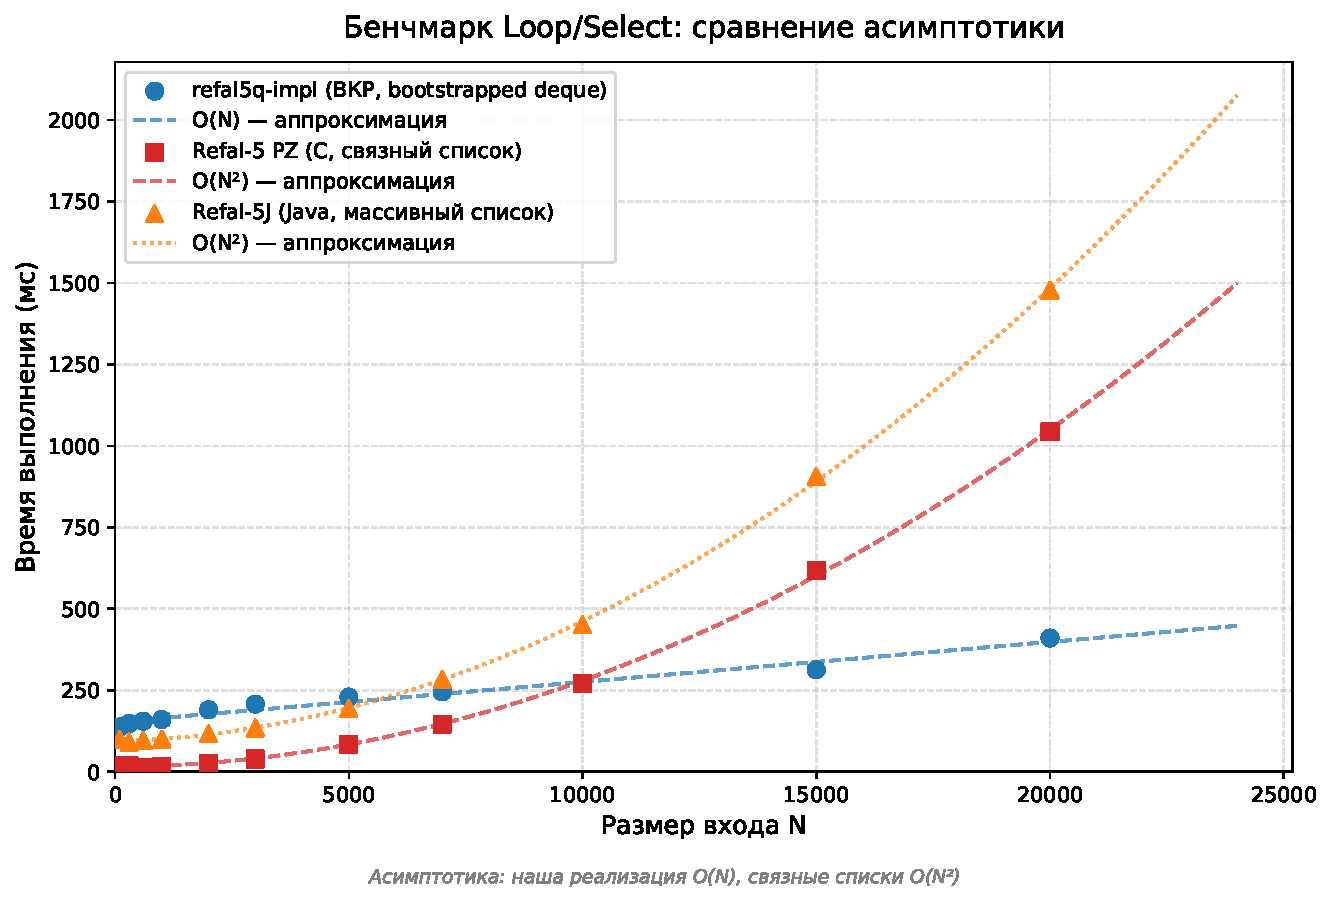
\includegraphics[width=0.95\textwidth]{loop-select-graph.pdf}
  \caption{Зависимость времени выполнения Loop/Select от размера входа N}
  \label{fig:bench-graph}
\end{figure}

\subsubsection{Тест на реальной программе: рассахариватель}

Loop/Select~--- синтетический тест: он нарочно нагружает ту единственную
операцию, на которой расходятся структуры данных. Чтобы проверить реализацию
на содержательной нагрузке, второй прогон выполнен на настоящей программе~---
рассахаривателе проекта \prog{refal-5-framework}~\cite{refal5_framework_github}.
Это пять модулей (\prog{desugar}, \prog{LibraryEx}, \prog{R5FW-Parser},
\prog{R5FW-Transformer}, \prog{R5FW-Plainer}) общим объёмом около 4200~строк;
на вход ему подаётся \prog{R5FW-Parser.ref}~--- сам синтаксический анализатор
рассахаривателя, 1038~строк, дающий на выходе около 45~КБ текста.

Один и тот же рассахариватель прогоняется тремя способами:
\begin{itemize}
  \item \prog{refal5q-impl}~--- наш интерпретатор исполняет пять
        рассахаренных \prog{.ref}-файлов напрямую;
  \item Refal-5~PZ~--- сначала компилирует \prog{.ref} в \prog{.rsl}
        (утилита \prog{refc}), затем исполняет (утилита \prog{refgo});
  \item Refal-5J~--- компилирует \prog{.ref} в \prog{.java}, затем в
        \prog{.class} (\prog{r5jc} + \prog{javac}) и запускает.
\end{itemize}

Все три реализации дают эквивалентный выход. Это и есть
главный результат теста: наш интерпретатор корректно исполняет реальную
программу такого объёма и воспроизводит поведение зрелых реализаций Рефала-5.

\subsubsection{Методика и результаты рассахаривателя}

Методика измерений совпадает с тестом Loop/Select: один прогревочный запуск
и три измеряемых, в отчёт идёт медиана. Для Refal-5~PZ и Refal-5J компиляция
выполняется один раз до замеров, поэтому измеряется только время исполнения
скомпилированной программы. Тайм-аут на один запуск~--- 300~секунд.

Запуск выполняется скриптом \prog{bench/desugar-bench.ps1}:

\begin{lstlisting}[language=bash,caption={Запуск бенчмарка рассахаривателя},label={lst:desugar-bench-run}]
powershell -File bench\desugar-bench.ps1 -WithPZ -WithR5J
\end{lstlisting}

Медианные времена приведены в таблице~\ref{tab:desugar-results}.

\begin{table}[!htb]
\caption{\centering Время рассахаривания R5FW-Parser.ref (мс, медиана 3 прогонов)}
\label{tab:desugar-results}
\centering
\small
\begin{tabular}{|l|r|l|}
\hline
\textbf{Реализация} & \textbf{Время, мс} & \textbf{Режим исполнения} \\
\hline
refal5q-impl & 2055 & интерпретация \\
\hline
Refal-5~PZ   & 369  & компиляция (refc + refgo) \\
\hline
Refal-5J     & 1632 & компиляция (r5jc + javac) \\
\hline
\end{tabular}
\end{table}

\subsubsection{Обсуждение результатов}

Два прогона отвечают на разные вопросы, поэтому обсудим их по очереди:
Loop/Select показывает, как ведёт себя структура данных под алгоритмической
нагрузкой, а рассахариватель~--- как реализация справляется с реальной
программой целиком.

Сначала о тесте Loop/Select.
На малых $N$ наша реализация проигрывает обоим конкурентам.
Причина простая: запуск JVM и прогрев JIT-компилятора стабильно стоят
около 120~мс, и эта плата не зависит от размера входа. Refal-5~PZ~---
нативный бинарник, его старт укладывается в единицы миллисекунд;
Refal-5J работает на той же JVM, что и мы, но тратит на инициализацию
порядка 85--90~мс.

При $N \approx 7000$ кривая Refal-5J уже догоняет нашу, при $N \approx 9000$
её перешагивает Refal-5~PZ. После этой точки квадратичный рост
конкурентов берёт своё: на $N = 10\,000$ PZ уже медленнее (277~мс против
254~мс), а на $N = 20\,000$ разрыв с PZ становится 3,5-кратным
(1059~мс против 302~мс) и 4,5-кратным с Refal-5J
(1348~мс против 302~мс).

Объяснение различия лежит в способе хранения объектного выражения.
Refal-5~PZ и Refal-5J держат выражение в виде двусвязного списка
термов: при построении нового скобочного терма \prog{(e.Acc A/B)}
на $k$-й итерации нужно скопировать всю накопленную часть длиной $k$.
$N$ итераций по $O(k)$ дают $O(N^2)$. Наш интерпретатор устроен иначе:
значение переменной идёт на стек одним объектом \prog{BulkPassive},
а сборка аргументов вызова использует \prog{Expr.concat}~--- по схеме
Окасаки это амортизированная константа независимо от длины операндов.
$N$ итераций по $O(1)$ дают $O(N)$~--- ровно то, что показывает прямая
на графике.

У замера есть границы применимости, и их стоит назвать прямо.
Меряется время жизни всего процесса, поэтому наши $\approx 120$~мс на $N = 100$~---
это почти целиком запуск JVM, а не работа интерпретатора. Диапазон $N$ до 20\,000
захватывает лишь начало параболы конкурентов: на больших $N$ разрыв рос бы быстрее, но
прогон при $N \sim 10^5$ уже упирается в тайм-аут 120~с. Наконец, PZ и Refal-5J в обоих
тестах выступают как компиляторы~--- компиляция сделана заранее, и замеряется только
исполнение готового кода, так что на Loop/Select мы сравниваем алгоритмические сложности
структур данных, а не режимы исполнения.

Теперь о тесте рассахаривателя.
И здесь конкуренты также работают как компиляторы: и Refal-5~PZ,
и Refal-5J сначала переводят программу в нативный код или байт-код, а потом
исполняют уже скомпилированное. Отличие от Loop/Select в том, что
рассахариватель не содержит квадратичного паттерна, поэтому алгоритмического
преимущества у нас нет, и они закономерно быстрее нашего интерпретатора~---
Refal-5~PZ в 5,6~раза, Refal-5J в 1,3~раза. Это не алгоритмический проигрыш,
а ожидаемая разница между компиляцией и интерпретацией: наша реализация на
каждом шаге заново разбирает поле зрения, тогда как скомпилированная программа
исполняет готовый код. Наибольший отрыв даёт Refal-5~PZ как нативный
компилятор; Refal-5J ближе к нам, потому что работает на той же JVM и платит
те же стартовые накладные расходы.

Важно, что главный вывод этого теста не про время, а про корректность: наш
интерпретатор исполняет программу в 4200~строк и выдаёт ровно тот же результат,
что зрелые реализации Рефала-5. Вместе два прогона дают согласованную картину.
На алгоритмически тяжёлом паттерне, где растущий аккумулятор многократно
копируется, выигрывает структура данных~--- раскрученная очередь даёт $O(N)$
там, где списочные представления дают $O(N^2)$. На обычной программе без
такого паттерна решает способ исполнения, и компиляция ожидаемо обходит
интерпретацию. Ни одно из наблюдений не противоречит другому: они измеряют
разные свойства реализации.
